\problemname{Cities}
In a far away kingdom, there are $N$ cities numbered between $0$ and $N - 1$.
The cities are connected by $N - 1$ two-way roads.
Each road has the same length, and connects exactly two cities, such that there is a unique path between any pair of cities.

For any two cities $A$ and $B$, denote by $L(A, B)$ the number of roads of this unique path between cities $A$ and $B$.
Given an integer $K$, for how many pairs of cities $A, B$ is $L(A, B) = K$?

\section*{Input}
The first line contains the integers $N$ and $K$ ($1 \le K \le N \le 100\,000$), described in the statement.

The two lines contains the $N - 1$ integers $f_1, \dots, f_{N-1}$ ($0 \le f_i < N$) and the $N - 1$ integers $t_1, \dots, t_{N-1}$ ($0 \le t_i < N$) respectively.
These describe the roads of the city: there is a road between city $f_i$ and $t_i$ for each $i$.

\section*{Output}
Output the number of pairs of cities that have exactly $K$ roads between them.


\section*{Scoring}
Your solution will be tested on a set of test groups, each worth a number of points.
To get the points for a test group you need to solve all test cases in the test group.

\noindent
\begin{tabular}{| l | l | l |}
  \hline
  Group & Points & Constraints \\ \hline
  $1$ & $9$ & $N \le 100$ \\ \hline
  $2$ & $19$ & $N \le 1\,000$ \\ \hline
  $3$ & $34$ & $K \le 10$ \\ \hline
  $4$ & $38$ & No additional constrsaints. \\ \hline
\end{tabular}

\section*{Explanation of sample 1}
Let the kingdom have $N = 5$ cities, connected by roads as in the figure below:
\begin{figure}[h!]
  \centering
  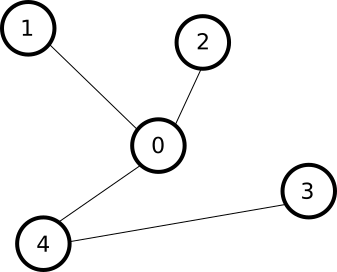
\includegraphics[width=0.3\textwidth]{sample.png}
  \caption{Illustration of the example}
\end{figure}

The following 4 pairs have a single road between them: $(0, 1), (0, 2), (0, 4), (3, 4)$.

The following 4 pairs have two roads between them: $(0, 3), (1, 2), (1, 4), (2, 4)$.

The following 2 pairs have three roads between them: $(1, 3), (2, 3)$.

This m
eans that if for $K = 1, 2, 3$, the answers would be $4, 4, 2$ respectively.
